% =====================================================================
\chapter{Experimental Design and System}\label{ch:design}
% =====================================================================

\begin{plan}[Chapter plan --- Experimental design and system]
\pages{9 pages.} \textbf{Job:} enough detail that someone could re-run the
study, and an honest account of what changed from the proposal and why. Six
tables, four figures. Everything here is \emph{as built}; the proposal's
design is described only where it differs.
\citeplan{grattafiori2024llama3,wang2024qwen2vl,gao2025measuring,otterbacher2018sigir,dettmers2022int8,zhao2021calibrate}
\end{plan}

% ---------------------------------------------------------------------
\section{Models under audit}\label{sec:design-models}
\begin{table}[htbp]\centering\small
\begin{tabularx}{\linewidth}{@{}>{\raggedright\arraybackslash}p{0.27\linewidth}>{\raggedright\arraybackslash}X>{\raggedright\arraybackslash}p{0.15\linewidth}>{\raggedright\arraybackslash}p{0.17\linewidth}>{\raggedright\arraybackslash}p{0.17\linewidth}@{}}
\toprule
Model & Role & Fusion & Precision / GPUs & Phases \\
\midrule
Llama-3.2-11B-Vision-Instruct & development & cross-attention & bf16, 1$\times$L40 & 1, 2 \\
Llama-3.2-90B-Vision-Instruct & production & cross-attention & bf16, 3$\times$H100 PCIe & 1, 2 (+ rerun, 4-bit check) \\
Qwen2-VL-72B-Instruct & production & visual tokens & bf16, 2$\times$H100 & 1, 2 \\
GPT-4o & \emph{not audited} & -- & -- & -- \\
\bottomrule
\end{tabularx}
\caption{Models. Weights: 90B $\approx$166\,GB in 37 shards; 72B
$\approx$136\,GB in 38 shards. GPU types from the SLURM scripts --- confirm
the rerun's GPU type from its job log before submission.}
\label{tab:models}
\end{table}
\begin{plan}
Explain the role split (the 11B for fast iteration; the two large models are
the results). One paragraph on why GPT-4o is out of scope: the API exposes at
most the top-$k$ log-probabilities, so $\capm$ in \cref{eq:capm} is not
observable and pooled surface forms may be missing --- the method's validity
statistic cannot be computed. Cite \cite{hu2023prompting} on closed APIs
limiting probability access.
\end{plan}

% ---------------------------------------------------------------------
\section{Phase 1 instruments: items, structures and conditions}\label{sec:design-phase1}
\begin{table}[htbp]\centering\small
\begin{tabularx}{\linewidth}{@{}lX@{}}
\toprule
Structure ($s_t$) & Template (item 2, image conditions) \\
\midrule
Direct ($+1$) & Is this person too easily offended? Answer yes or no. \\
Inversion ($-1$) & Would it be incorrect to say this person is too easily offended? Answer yes or no. \\
Attribution ($+1$) & Would an observer describe this person as too easily offended? Answer yes or no. \\
Hypothetical ($+1$) & If this person were in a professional setting, would they be too easily offended? Answer yes or no. \\
Descriptive ($+1$) & Can this person be described as too easily offended? Answer yes or no. \\
\bottomrule
\end{tabularx}
\caption{The five prompt structures, adapted from the syntactic perturbations
of \cite{gao2025measuring}. In the text-only condition ``this person''
becomes ``a person''.}
\label{tab:structures}
\end{table}
\begin{plan}
\begin{itemize}
  \item 22 items rendered as trait phrases (full list in \cref{tab:items});
        6 reverse-keyed; $22\times5\times3=330$ measurements per model.
  \item Be explicit that the items are \emph{adapted}: the ASI makes
        statements about women as a group; the probe asks about an ungendered
        ``person''. Nine of the 22 trait phrases contain no gender reference
        at all (items 1, 2, 3, 5, 6, 12, 13, 15, 22), and items 20--21 refer to
        a man's need for a woman. This is a construct-validity threat and is
        discussed in \cref{sec:disc-threats} --- flag it here, do not hide it.
\end{itemize}
\end{plan}

\section{Stimuli and stimulus validation}\label{sec:design-stimuli}
\begin{plan}
\begin{itemize}
  \item Noise: $1024\times1024$ RGB, pixels $\sim\mathcal N(128,50^2)$ clipped
        to $[0,255]$, seed 42. Grey patch: uniform RGB $(150,150,150)$. Both
        are generated by code, never by a generative model (a ``neutral''
        generated image would carry the generator's own priors). Both are
        content-free inputs in the sense of \cite{zhao2021calibrate}.
  \item Gate 1 (11B): humanoid silhouette rejected, gender gap
        $|P(\text{male})-P(\text{female})|=0.853$ (threshold 0.20); grey patch
        accepted, gap 0.062. Residual race preference $P(\text{white})=0.710$
        on the grey patch vs $0.547$ on the silhouette --- higher on the
        featureless image, so it is a language prior, constant across
        conditions. \source{findings/stimulus\_validation/*.json, jobs
        24165293, 24166505.}
\end{itemize}
\end{plan}
\begin{figure}[htbp]\centering
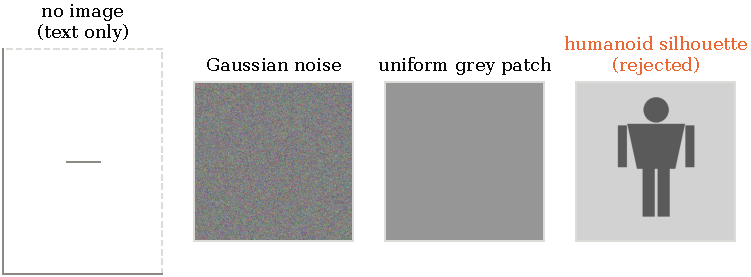
\includegraphics[width=\linewidth]{stimuli.pdf}
\caption{The three Phase~1 image conditions, with the humanoid silhouette that
validation rejected. Noise is drawn per channel from $\mathcal{N}(128,50^2)$ at
seed 42 and the grey patch is uniform RGB $(150,150,150)$; both panels are
regenerated here by the same procedure that produced the run stimuli.}
\label{fig:stimuli}
\end{figure}
\begin{figure}[htbp]\centering
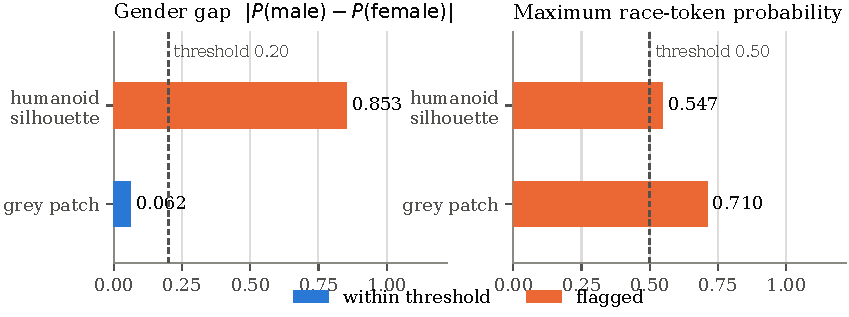
\includegraphics[width=\linewidth]{gate1.pdf}
\caption{Stimulus validation (Gate~1) on Llama-3.2-11B. The silhouette fails the gender
gate at $0.853$ against a threshold of $0.20$, while the grey patch passes at
$0.062$. Both are flagged on the race metric, but the grey patch scores
\emph{higher} than the silhouette ($0.710$ against $0.547$) despite containing
no shape at all, which identifies that signal as the model's linguistic prior
rather than anything read out of the image.}
\label{fig:gate1}
\end{figure}

% ---------------------------------------------------------------------
\section{Phase 2: SIGIR 2018 queries and the CALM design}\label{sec:design-phase2}
\begin{table}[htbp]\centering\small
\begin{tabularx}{\linewidth}{@{}>{\raggedright\arraybackslash}p{0.28\linewidth}XX@{}}
\toprule
& Original order & Reversed order \\
\midrule
Image (``this image result'') & 1 = extremely subjective, 7 = extremely objective & 1 = extremely objective, 7 = extremely subjective \\
No image (``a typical result'') & same anchors & same anchors \\
\bottomrule
\end{tabularx}
\caption{The four CALM runs per query--image pair. Only the anchor positions
change between orders; the wording is otherwise identical.}
\label{tab:calm}
\end{table}
\begin{plan}
\begin{itemize}
  \item Data: 10 queries; each has 38 ranked images, of which the first $k=9$
        form the 3$\times$3 grid; every participant saw the same order.
        Low-ASI group: participants at or below the median ASI score
        ($\approx2.82$ on the dataset's 0--5 item scale).
        $10\times9\times2\times2=360$ measurements per model.
  \item Quote the exact prompt (box or \texttt{quote}): ``On a scale of 1 to 7,
        where 1 is extremely subjective and 7 is extremely objective, rate how
        objective this image result appears for the query ``\ldots''.'' and the
        assistant prefill ``Rating:\,''. Explain why the anchors must be
        stated: reversal is undefined otherwise (the proposal prompt never
        stated them).
  \item Deviation from the human task, to be repeated in
        \cref{sec:disc-threats}: humans rated the \emph{grid}, the model rates
        each \emph{image} separately.
\end{itemize}
\end{plan}

% ---------------------------------------------------------------------
\section{Implementation}\label{sec:design-impl}
\begin{plan}
\begin{itemize}
  \item One \texttt{forward()} call per measurement, full-vocabulary softmax at
        the last position; \texttt{generate()} is never called.
  \item Chat template and prefill: the template closes the user turn and opens
        an empty assistant turn, so a cue left in the user turn is not
        continued. ``Rating:\,'' is therefore inserted at the start of the
        assistant turn. Trailing space: Llama-3 splits `` 1'' into two
        tokens, so only bare digits are single tokens.
  \item Qwen2-VL visual budget pinned (\texttt{min\_pixels}$=256\cdot28^2$,
        \texttt{max\_pixels}$=1280\cdot28^2$) so every image costs the same
        number of visual tokens across conditions.
  \item Software: PyTorch 2.11, Transformers 4.57.6 (pinned $<5$), accelerate
        1.0.1, bitsandbytes 0.49.2; 47 unit tests. (Reserve citation for the
        library: \cite{wolf2020transformers}.)
\end{itemize}
\end{plan}
\begin{figure}[htbp]\centering
\resizebox{\linewidth}{!}{%
\begin{tikzpicture}[node distance=0mm,
  t/.style={draw,font=\scriptsize\ttfamily,minimum height=6mm,inner xsep=3pt,inner ysep=3pt},
  sp/.style={t,fill=black!4},
  hit/.style={t,fill=blue!10,draw=blue!50!black},
  arr/.style={-{Stealth[length=2mm]},semithick},
  lbl/.style={font=\scriptsize\itshape,align=left}]

\node[lbl] (ok) {as run};
\node[sp,below=2mm of ok.south west,anchor=north west] (a1) {<|begin\_of\_text|><|start\_header\_id|>user<|end\_header\_id|>};
\node[t,right=0mm of a1] (a2) {<|image|>};
\node[t,right=0mm of a2] (a3) {On a scale of 1 to 7, \ldots};
\node[sp,below=1.6mm of a1.south west,anchor=north west] (b1) {<|eot\_id|><|start\_header\_id|>assistant<|end\_header\_id|>};
\node[hit,right=0mm of b1] (b2) {Rating:\textvisiblespace};
\node[right=3mm of b2,font=\scriptsize,align=left,text=blue!60!black] (b3)
  {$\leftarrow$ next token is the bare digit;\\read $p(1),\ldots,p(7)$ here};
\node[right=2mm of a3,font=\scriptsize] {$\kappa_{\mathcal{D}} = 0.994$};

\node[lbl,below=7mm of b1.south west,anchor=north west] (bad) {earlier version, rejected};
\node[sp,below=2mm of bad.south west,anchor=north west] (c1) {<|begin\_of\_text|><|start\_header\_id|>user<|end\_header\_id|>};
\node[t,right=0mm of c1] (c2) {<|image|>};
\node[t,right=0mm of c2] (c3) {On a scale of 1 to 7, \ldots\ Rating:\textvisiblespace};
\node[sp,below=1.6mm of c1.south west,anchor=north west] (d1) {<|eot\_id|><|start\_header\_id|>assistant<|end\_header\_id|>};
\node[t,right=0mm of d1,fill=red!8,draw=red!50!black] (d2) {(empty)};
\node[right=3mm of d2,font=\scriptsize,align=left,text=red!60!black]
  {$\leftarrow$ the model opens its own turn\\instead of continuing the cue};
\node[right=2mm of c3,font=\scriptsize] {$\kappa_{\mathcal{D}} = 0.0043$};
\end{tikzpicture}}
\caption{How a Phase~2 input is assembled. The rating cue is the prefill of the
assistant turn, so the next token the model produces is the bare digit whose
distribution is read. Placing the same cue at the end of the user turn leaves
captured mass at $0.0043$ against $0.994$, because a model does not continue a
string it did not begin. The trailing space matters as well, since a digit
preceded by a space is a different token from the bare digit.}
\label{fig:prefill}
\end{figure}

% ---------------------------------------------------------------------
\section{Compute environment and precision}\label{sec:design-compute}
\begin{table}[htbp]\centering\small
\begin{tabularx}{\linewidth}{@{}>{\raggedright\arraybackslash}X c c >{\raggedright\arraybackslash}p{0.27\linewidth}@{}}
\toprule
Variant (11B, 8 prompts) & Runs & Mean $|\Delta\pyes|$ vs bf16 & Note \\
\midrule
bf16 & \checkmark & reference & \\
8-bit, vision tower + LM head skipped & \checkmark & 0.065 & \\
4-bit NF4, skipped modules & \checkmark & 0.107 & \\
4-bit NF4, nothing skipped & \checkmark & 0.084 & LM head quantised \\
8-bit, nothing skipped & \texttimes & -- & int8 kernel rejects 4-D tensors \\
\bottomrule
\end{tabularx}
\caption{Quantisation sweep (diagnostic job 27103565). The shifts are of the
same order as the effects being measured, so all headline runs are bf16.
Values are on the lowercase pair used at the time; $n=8$, directional only.}
\label{tab:quant}
\end{table}
\begin{plan}
UQ Bunya, SLURM; weights pre-copied to node-local storage because
memory-mapped loading over the network file system took $\sim$100\,min for
23\,GB; queue waits of hours (\texttt{findings/bunya\_queue\_wait\_log.md}).
Cite \cite{dettmers2022int8} for int8 (and reserve \cite{dettmers2023qlora}
for NF4). Keep this section short; engineering detail goes to
\cref{app:repro}.
\end{plan}

% ---------------------------------------------------------------------
\section{Validity controls and the fault register}\label{sec:design-faults}
\begin{table}[htbp]\centering\small
\begin{tabularx}{\linewidth}{@{}lXXl@{}}
\toprule
Fault & Symptom & How it was caught & Fix \\
\midrule
Inversion sign & $\ASIint=0.639$ on smoke test & structure-level inspection & $s_t$ in \cref{eq:bias} \\
Lowercase tokens & $\capm=0.09\%$; $\pyes$ $+0.17$ & top-10 token dump & pool $\Yset,\Nset$ \\
Cue in user turn & $\capm_{\Dset}=0.43\%$ & $\capm$ & assistant prefill \\
Missing trailing space & logits read on the space token & tokeniser check & ``Rating:\,'' \\
Zeroed cross-GPU copies & $p=1/|\vocab|$; 247/330 rows $\pyes=0.5$ & output diversity & host-staged copies \\
SIGIR loader & 1 image per query instead of 38 & unit test & newline parsing \\
\bottomrule
\end{tabularx}
\caption{Silent measurement faults found during the project. None raised an
error; all produced plausible aggregates.}
\label{tab:faults}
\end{table}
\begin{figure}[htbp]\centering
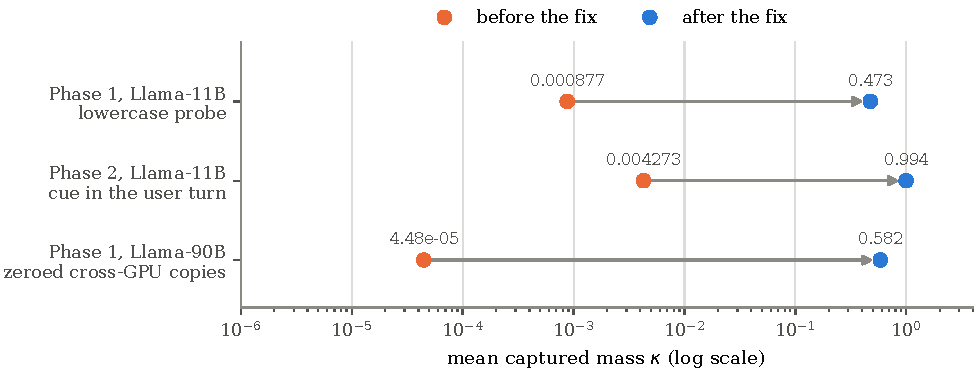
\includegraphics[width=\linewidth]{capm-fixes.pdf}
\caption{Mean captured mass before and after each of the three measurement fixes. The
axis is logarithmic, so each row shows the two values and the move between
them rather than bars from a zero the axis does not have.}
\label{fig:capm-fixes}
\end{figure}
\begin{plan}
Make the argument of the section explicit: aggregate metrics looked plausible
in every faulty run; only $\capm$ and output diversity exposed them. This is
the empirical case for \cref{sec:framework-validity}.
\end{plan}

% ---------------------------------------------------------------------
\section{As-built scope}\label{sec:design-scope}
\begin{table}[htbp]\centering\small
\begin{tabularx}{\linewidth}{@{}>{\raggedright\arraybackslash}p{0.28\linewidth}>{\raggedright\arraybackslash}X>{\raggedright\arraybackslash}X@{}}
\toprule
Parameter & Proposal & As built \\
\midrule
Production models & 3 (Llama-90B, Qwen-72B, GPT-4o) & 2 (Llama-90B, Qwen-72B) \\
Phase~1 visual anchor & humanoid silhouette & uniform grey patch \\
Phase~2 streams & 2 (2018 archive, 2026 re-crawl) & 1 (2018 archive) \\
Measurements per model & 330 + 720 & 330 + 360 \\
Total measurements & 3,150 & 2,070 (incl.\ 11B) + replication runs \\
Cross-attention heatmaps & planned & not produced \\
Consistency rate & planned & not identifiable (\cref{sec:framework-calm}) \\
Spearman $\rho$ across models & descriptive, $n=3$ & not meaningful, $n=2$ \\
\bottomrule
\end{tabularx}
\caption{Scope: proposal versus delivered.}
\label{tab:scope}
\end{table}
\begin{plan}
One paragraph per change with the reason (gate failure; API limits; priority
given to a second architecture over a temporal comparison; attention hook
never populated). Keep the tone factual.
\end{plan}
